\pdfoutput=1
% \documentclass[draft, a4paper, 12pt]{article}
% \usepackage[margin={1.25cm,2.5cm}]{geometry}

%= PAGE/CONTENT SIZE
\documentclass[letterpaper, 12pt]{article}
\usepackage[top=0.50in,bottom=0.75in,left=15mm,right=15mm]{geometry}

%= FONT FAMILY
\fontfamily{ptm}\selectfont

%= FIGURES & GRAPHICS
\usepackage{graphicx}
\graphicspath{{figures/}}
\usepackage{floatrow}
\usepackage{wrapfig}
\usepackage{soul}
\usepackage{subfigure}
\usepackage{dblfloatfix}

%= HYPER
\def\UrlBreaks{\do\/\do-}

%= BIBLIOGRAPHY
\usepackage[backend=bibtex,style=alphabetic,
            bibencoding=ascii,sorting=ynt]{biblatex}
\addbibresource{bibliography}

%= BETTER MATH
\usepackage{amssymb}
\usepackage{amsmath}
\usepackage{pst-node}
\usepackage{cases}

%= LOREM IPSUM
\usepackage{lipsum}

%%%%%%%%%%%%%%%%%%%%%%%%%%%%%%%%%%%%%%%%%%%%%%%%%%%%%%%%%%%%%%%%%%%%%%%%%%%%%%%%%
%% FIXES
%%%%%%%%%%%%%%%%%%%%%%%%%%%%%%%%%%%%%%%%%%%%%%%%%%%%%%%%%%%%%%%%%%%%%%%%%%%%%%%%%

% #1 : DOT AFTER SECTION
\usepackage{titlesec}
\titlelabel{\thetitle. }

% #2 : CODE/SNIPPETS APPENDIX
\usepackage{algorithm2e}
\usepackage{listings}
\usepackage{inconsolata}

\lstset{language=python}
\lstset{linewidth=\columnwidth}

\usepackage{color}
\usepackage{xcolor}
\definecolor{lightgray}{rgb}{.9,.9,.9}
\definecolor{darkgray}{rgb}{.4,.4,.4}
\definecolor{purple}{rgb}{0.65, 0.12, 0.82}

\lstdefinelanguage{python}{
keywords={False, None, True, and, as, assert, break, class, continue, def, del,
elif, else, except, finally, for, from, global, if, import, in, is, lambda,
nonlocal, not, or, pass, raise, return, try, while, with, yield},
keywordstyle=\color{blue}\bfseries,
ndkeywords={return, class, if ,elif, endif, while, do, else, True, False ,
catch, def, boolean, throw, import},
ndkeywordstyle=\color{darkgray}\bfseries,
identifierstyle=\color{black},
sensitive=false,
comment=[l]{\#},
morecomment=[s]{/*}{*/},
commentstyle=\color{purple}\ttfamily,
stringstyle=\color{red}\ttfamily,
morestring=[b]',
morestring=[b]"
}

\lstset{
language=python,
extendedchars=true,
basicstyle=\footnotesize\ttfamily,
showstringspaces=false,
showspaces=false,
tabsize=2,
breaklines=true,
showtabs=false,
captionpos=b,
upquote=true,
columns=flexible,
keepspaces=true,
fontadjust=true
}

\makeatletter
\def\lst@outputspace{{\ifx\lst@bkgcolor\empty\color{white}
\else\lst@bkgcolor\fi\lst@visiblespace}}
\makeatother

% #3 : LIST MARGIN
\usepackage{enumitem}
\setlist[itemize]{leftmargin=4mm}

% #4 : THEOREM
\newtheorem{theorem}{Theorem}[section]
\newtheorem{corollary}{Corollary}[theorem]
\newtheorem{lemma}[theorem]{Lemma}

% #5 : QUOTES
\usepackage{csquotes}

%%%%%%%%%%%%%%%%%%%%%%%%%%%%%%%%%%%%%%%%%%%%%%%%%%%%%%%%%%%%%%%%%%%%%%%%%%%%%%%%%
%% VARIABLES
%%%%%%%%%%%%%%%%%%%%%%%%%%%%%%%%%%%%%%%%%%%%%%%%%%%%%%%%%%%%%%%%%%%%%%%%%%%%%%%%%

\usepackage[pdftex,
pdfauthor={Maciej A. Czyzewski},
pdftitle={An Extremely Efficient Chess-board Detection for Non-trivial Photos},
pdfkeywords={chess-board detection/localization, chess-board corner detection,
feature extraction, pattern recognition, photogrammetric marker detection, board
recognition, implementation},
pdfsubject={computer vision, machine learning}]{hyperref}

%= TITLE
\title{\fontsize{18.5}{14.4}\textbf{\MakeUppercase{%
An Extremely Efficient Chess-board Detection for Non-trivial Photos}}}

%= AUTHOR
\author{
  Maciej A. Czyzewski\\
  \texttt{mail@maciejczyzewski.me}
}

\begin{document}

\maketitle

%%%%%%%%%%%%%%%%%%%%%%%%%%%%%%%%%%%%%%%%%%%%%%%%%%%%%%%%%%%%%%%%%%%%%%%%%%%%%%%%%
%%%%%%%%%%%%%%%%%%%%%%%%%%%%%%%%%%%%%%%%%%%%%%%%%%%%%%%%%%%%%%%%%%%%%%%%%%%%%%%%%
%%                            BEGIN OF DOCUMENT                                %%

\noindent\textbf{Abstract.} 
We present a set of algorithms that can be used to locate and crop the chess-board/chess-pieces from the picture, including every rectangular grid with any pattern.
Our method is non-parametric, and thus does not require the prior knowledge from
computer vision and machine learning, which is instead inferred from data.
We illustrate the application of our method to a variety of examples, such as
chess-board cropping and regular grid-pattern localization.
In addition, we present two independent algorithms: PAMG (vertices detector) and
FAPL (thermal lines) that can be widely used for other tasks in computer vision.
\newline\newline
\noindent\textbf{Keywords.} chess-board detection/localization $\cdot$ chess-board corner detection $\cdot$ feature extraction $\cdot$ pattern recognition $\cdot$ photogrammetric marker detection $\cdot$ board recognition $\cdot$ implementation
\newline\newline
\noindent\textbf{Project.} \hfill
\href{http://github.com/maciejczyzewski/neural-chessboard}{\textbf{github.com/maciejczyzewski/neural-chessboard}}

%%%%%%%%%%%%%%%%%%%%%%%%%%%%%%%%%%%%%%%%%%%%%%%%%%%%%%%%%%%%%%%%%%%%%%%%%%%%%%%%%
%% INTRODUCTION
%%%%%%%%%%%%%%%%%%%%%%%%%%%%%%%%%%%%%%%%%%%%%%%%%%%%%%%%%%%%%%%%%%%%%%%%%%%%%%%%%

\section{Introduction}

Everyone knows how to crop a chess-board from a photograph.
Typing to any search engine ``chess-board crop using computer vision'', we
get a lot of results. It shows out that most of these methods do their job very
badly. That is why we decided to take up this topic again.

In addition, we present method of cropping every rectangular grid with any
pattern. However, in this paper we will focus on chess-boards, especially for different types and scenarios.
The whole cutting process has been designed to be fast and simple in
implementation\footnote{for someone with a basic knowledge of computer vision and machine learning}.

Our method uses an experimental self-learning chess-board vertices detector named
PAMG with embedded neural network, which is the direct successor of the ChESS detector \cite{DBLP:journals/corr/abs-1301-5491}.
Both detectors achieve the same results for most images, but PAMG does better in
extreme cases\footnote{explanation is presented in conclusion}.

However, we should warn that \ul{PAMG and FAPL are only a drafts, in further work
we intend to describe them in detail}. In this paper we could safely
substitute FAPL with the CannyLines algorithm \cite{lu2015cannylines}, and PAMG
with the PTAM or ChESS algorithm. The results and effectiveness would probably be similar.

\section{Problem Description}

The main goal is to indicate the method for locating and cropping the
chess-board from the picture, which could be used later to create a digital record of the chess position using Forsyth-Edwards notation \cite{edwards1994portable}.
An additional goal was to design a successor to the ChESS detector, which is the
successor of the PTAM detector \cite{klein2007parallel}.
Our detector can be easily modified to detect other patterns, not only chess
corners, and by changing the process itself, there is a possibility to crop every rectangular grid with any pattern.

We also relied on the ease of implementation. After reading this paper, using
ready-made tools such as \textbf{Opencv} and \textbf{Tensorflow}, the
implementation should not take more than 2 hours. Ready to use implementation is
available here: \url{https://github.com/maciejczyzewski/neural-chessboard}

\section{Related Work}

\begin{wrapfigure}{R}{0.25\textwidth}
\centering\vspace*{-0.25in}
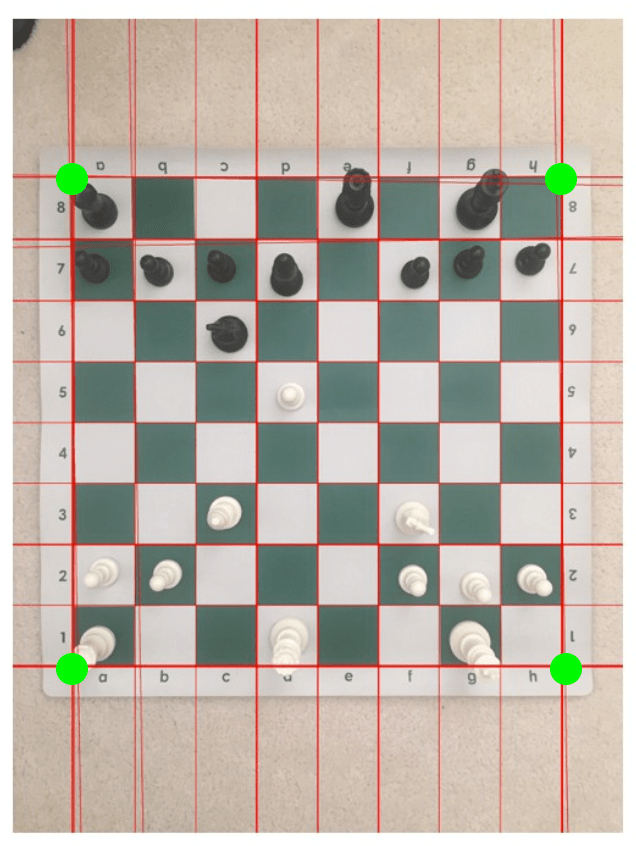
\includegraphics[width=\columnwidth]{figure1.png}
\caption{visualization of the method used in \textbf{daylen/chess-id} project}
\end{wrapfigure}

Most of the previous computer vision work related to chess has focused on the
area of board recognition. Many projects on \textbf{Github} proposes their own methods, these projects are mostly designed to digitize chess games. At the professional
level, specialized chess sets\footnote{for example \textbf{DGT e-Boards}} have been developed to record moves automatically.
However, this equipment is expensive and not easily accessible to recreational
players. Thus, people prefers computer vision, because a good quality
cameras can be found everywhere and they are obviously cheap.

Unfortunately, many of these methods are not universal. We know from the
experience \ul{that they mostly use the bird's eye view, where the central
object is a chess-board}\footnote{we have checked almost all projects published
on Github, the best \url{https://github.com/daylen/chess-id} passed barely 25\%
our test cases}.
Some of them have naive assumptions, leading to absurdity.

Stuart Bennett and Joan Lasenby, who created a well-functioning ChESS detector,
have done a milestone jump in the field of corner detection.
However, to get the chess-board out, more important is the method rather than
the feature detector. Thus, in this work we have focused on the method and process.

\section{Framework}

General techniques for board recognition can be separated into corner-based
approaches and line-based approaches, our method is a mix of them. Additionally,
we use something what we called facetiously
``deep analysis'', because the algorithm finds chess-board more and more closer
by passing the layers.

\subsection{Method}

\begin{figure}[H]
\centering
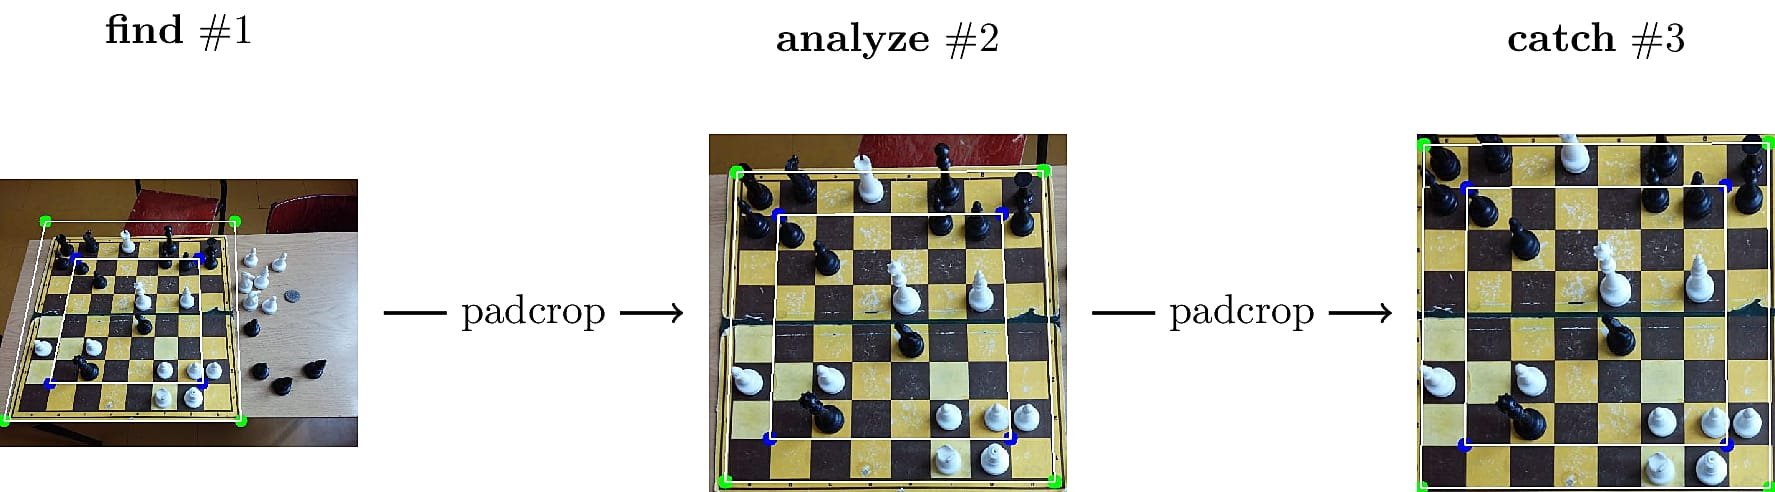
\includegraphics[width=0.8\columnwidth]{figure2}
\caption{deep analysis predominantly consists of 3 layers}
\end{figure}

The method is divided into three layers which seem to mimic a natural mental
process, that human brain is doing in natural environment:

\begin{itemize}

\item\textbf{find} \#1: chess-board localization (here, accuracy does not count)

\item\textbf{analyze} \#2: detect chess-board corners (almost perfect)

\item\textbf{catch} \#3: improve point matching (according to the perspective)

\end{itemize}

\subsection{Layer}

\begin{figure}[H]
\centering
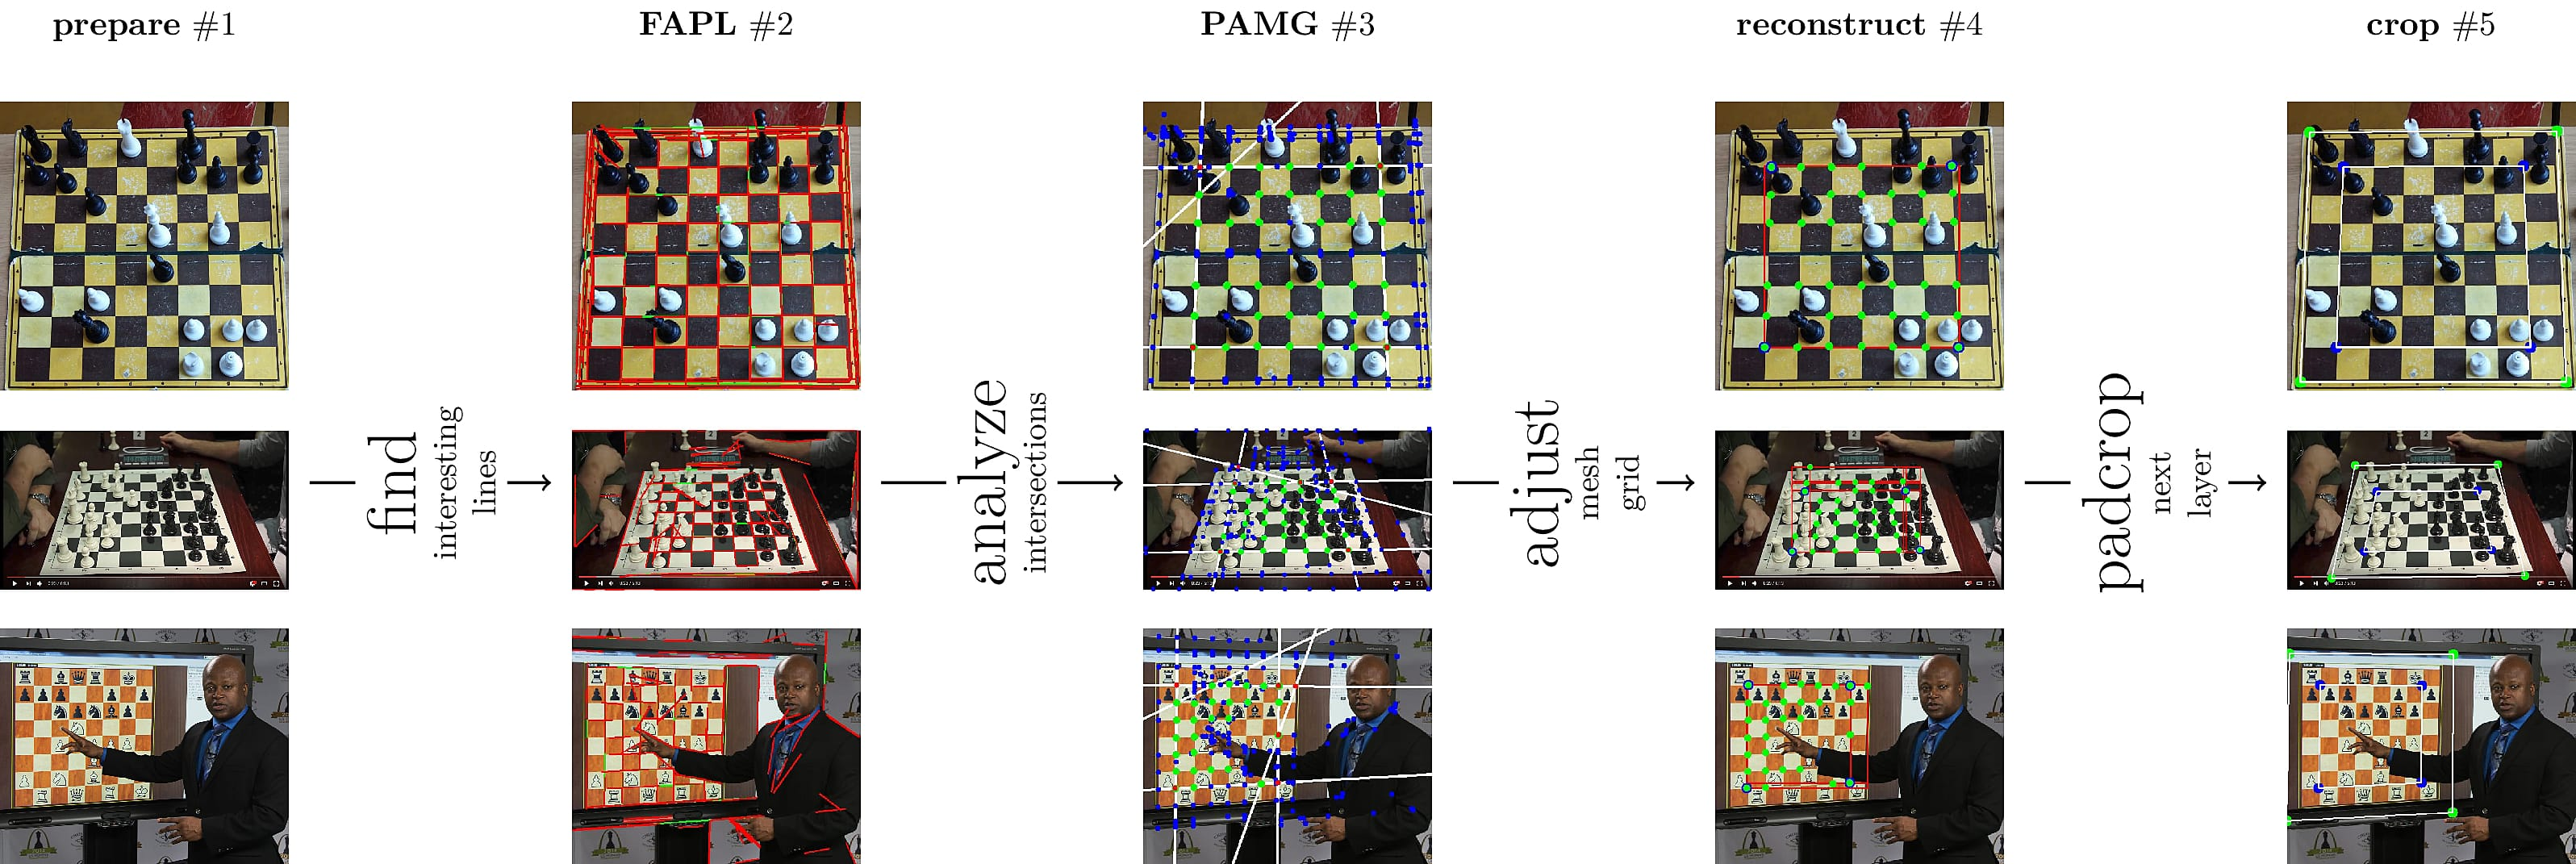
\includegraphics[width=\columnwidth]{figure3}
\caption{each layer has 5-step analysis}
\end{figure}

At each stage we will use the same block of operations:

\begin{itemize}

\item\textbf{prepare} \#1: prepare photo - ex. repair colors using
\textit{retinex} algorithm

\item\textbf{FAPL} \#2: apply algorithm - \textbf{f}ind \textbf{a}ll
\textbf{p}ossible \textbf{l}ines

\item\textbf{PAMG} \#3: apply algorithm - \textbf{p}otentially \textbf{a}
\textbf{m}esh \textbf{g}rid

\item\textbf{reconstruct} \#4: reconstruct a last layer of grid using previous data

\item\textbf{crop} \#5: crop a photo with a padding around $\,\to\,$ \textit{go to the first step}

\end{itemize}

\subsection{FAPL}

\begin{figure}[H]
\centering
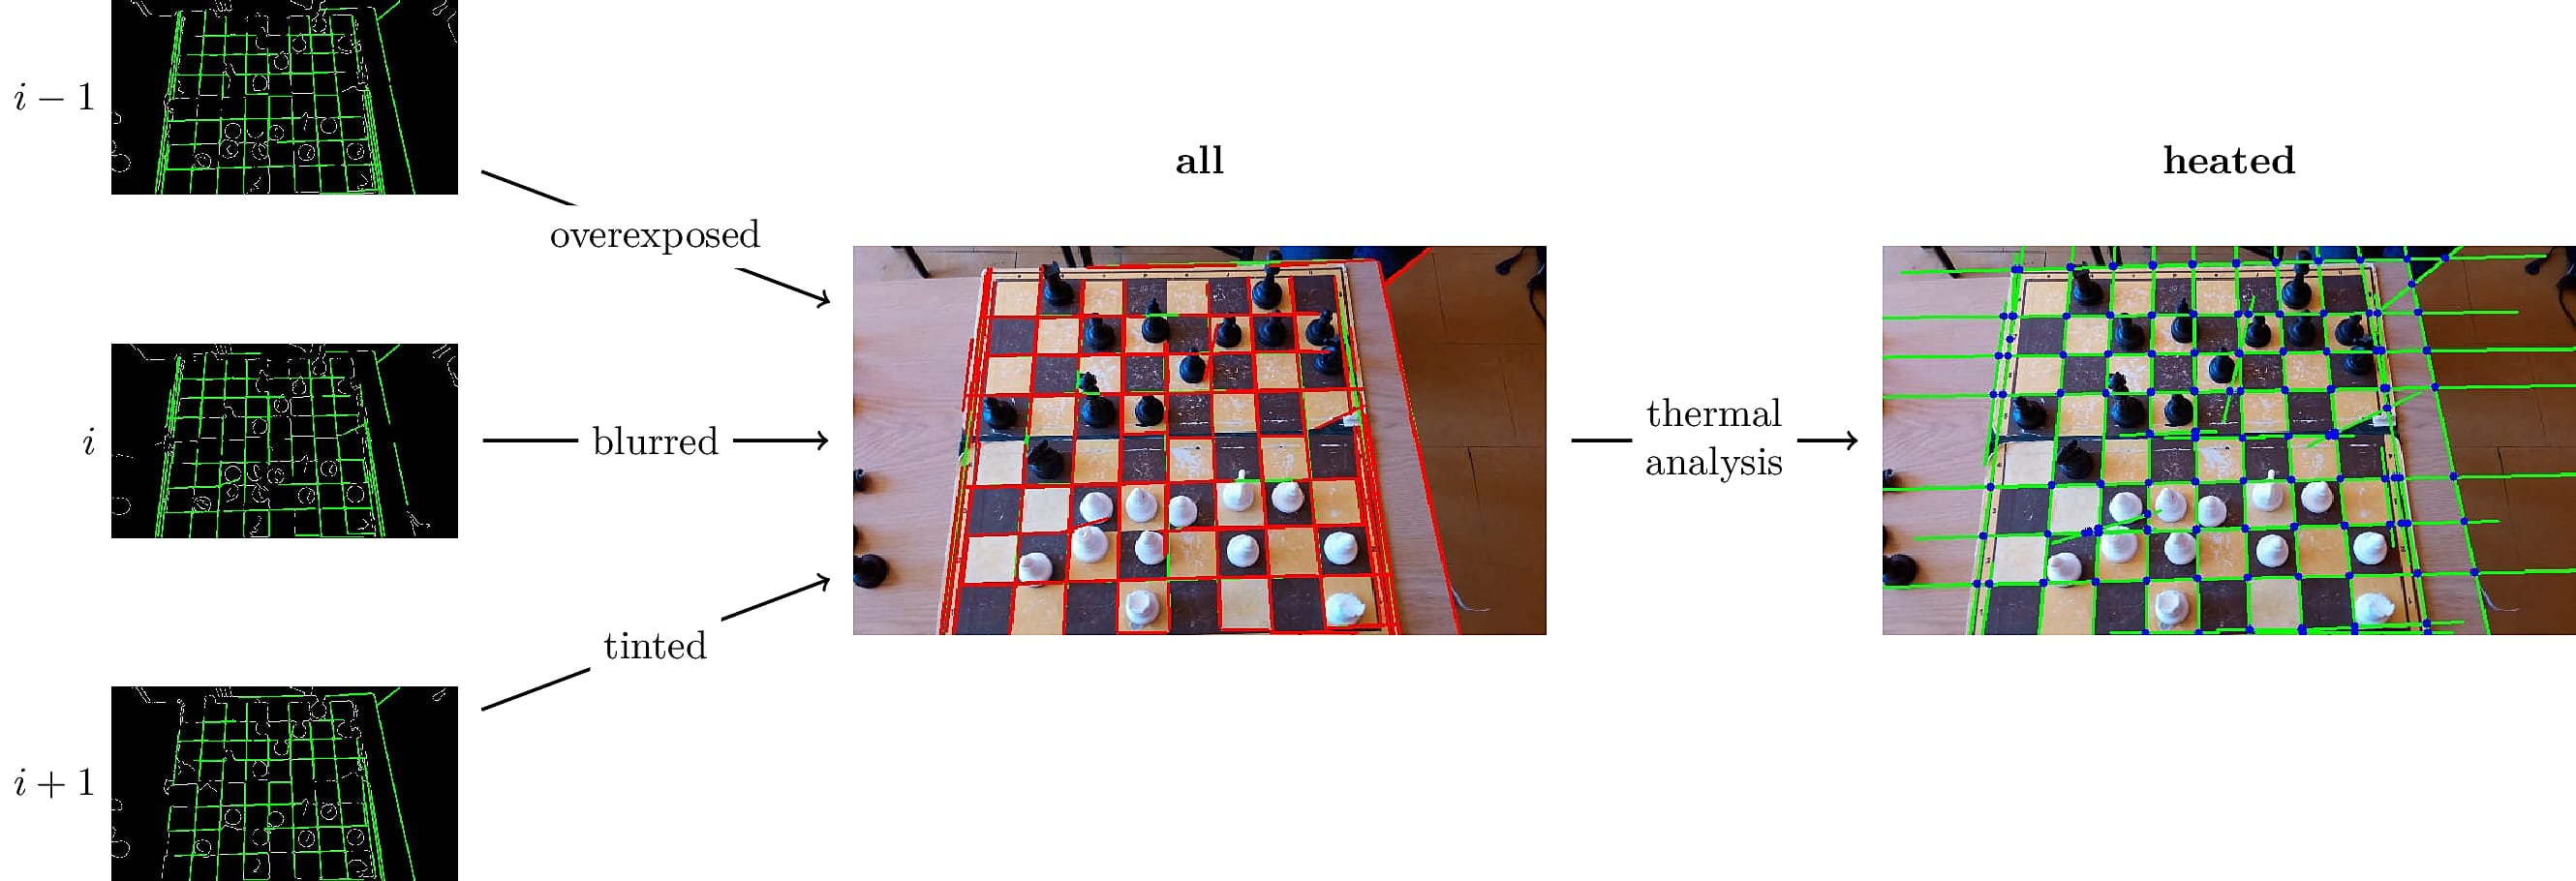
\includegraphics[width=\columnwidth]{figure4}
\caption{visualization how FAPL detects lines}
\end{figure}

The FAPL module detects all lines that are interesting for further analysis, even when the line is fragmented and not clearly defined.
The first step is to create multiple versions of the same image with different
defects, such as illumination, darkening.
In our algorithm we obtained this effect by choosing different parameters for
the threshold and CLAHE (adaptive histogram equalization
\cite{reza2004realization}).
The next step is to create a probabilistic thermal map of the found
segments\footnote{we recommend 2d-quadtree if you want to implement it}.
In area where segments overlaps, thermal map is hotter than in places where they occurs only few times.
The last step is to analyze the warmth of the local area by gradually connecting the common or close segments.
When we get to some fixed ``curiosity'' level, we stop the process.

\begin{figure}[H]
\centering
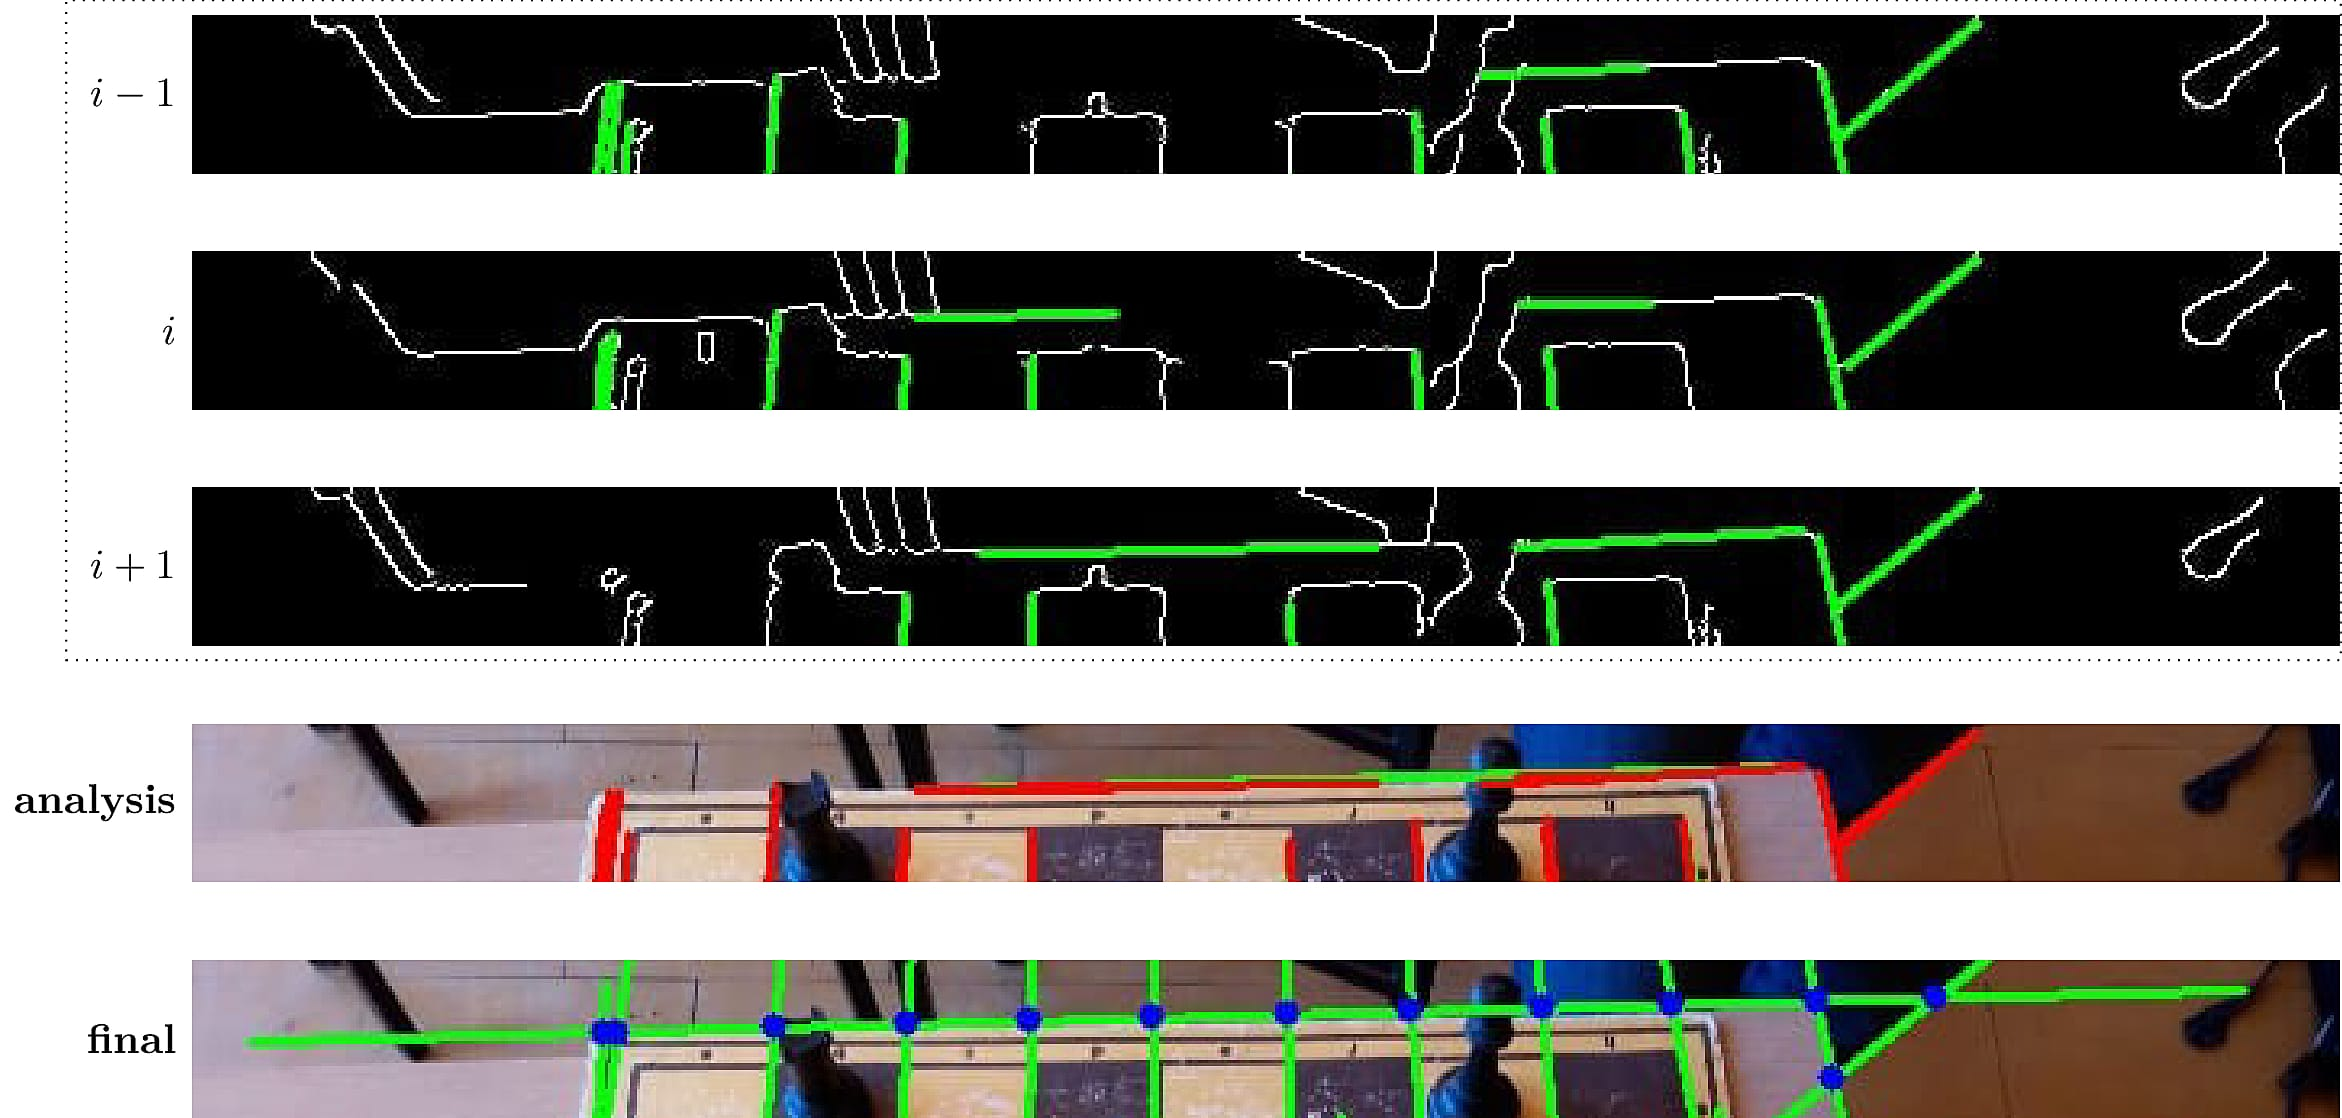
\includegraphics[width=\columnwidth]{figure5}
\caption{example of line that Hough line transform would not find using single input image}
\end{figure}

\subsection{PAMG}

The PAMG module is a self-learning two-piece detector for detecting the lattice
points of a chess-board.
The detector consists of a neural network and a geometric classifier. Both elements live together in symbiosis.
Geometric classifier recognizes only perfect cases.
The neural network recognizes deformed and distorted patterns.

\begin{figure}[H]
\centering
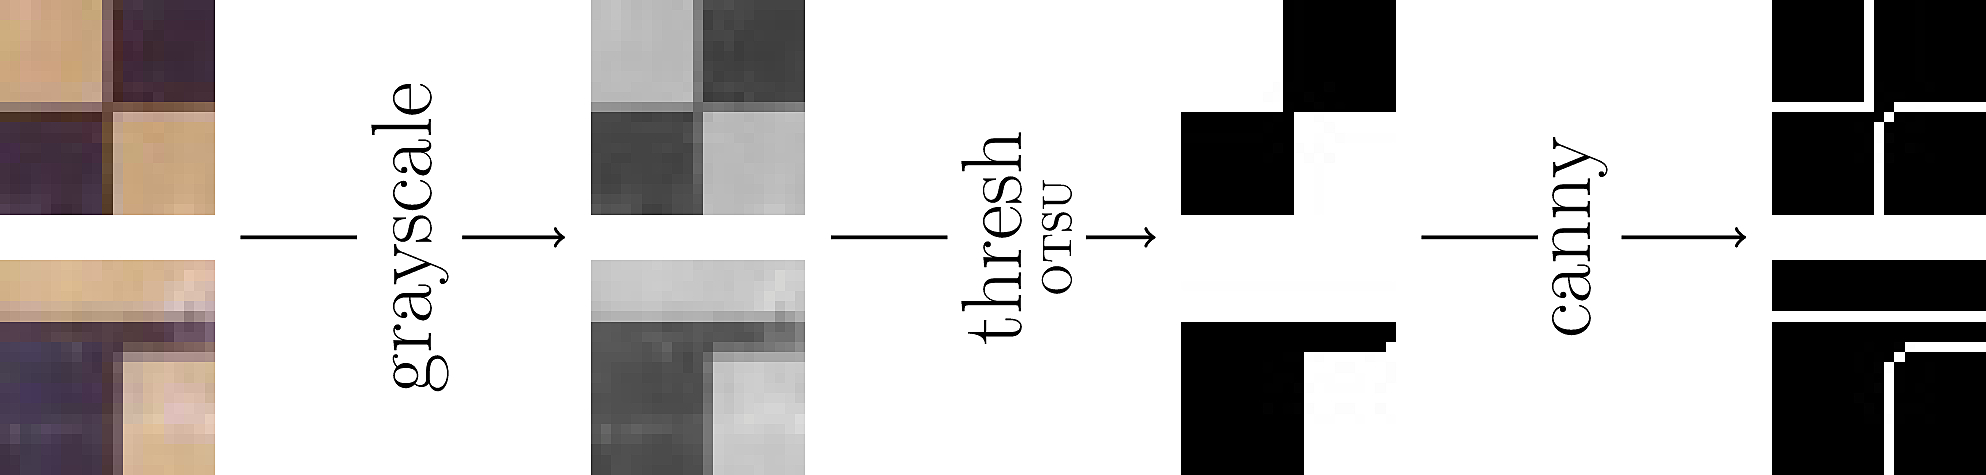
\includegraphics[width=\columnwidth]{figure6}
\caption{preparing image for the detector}
\end{figure}

\begin{figure}[H]
\centering
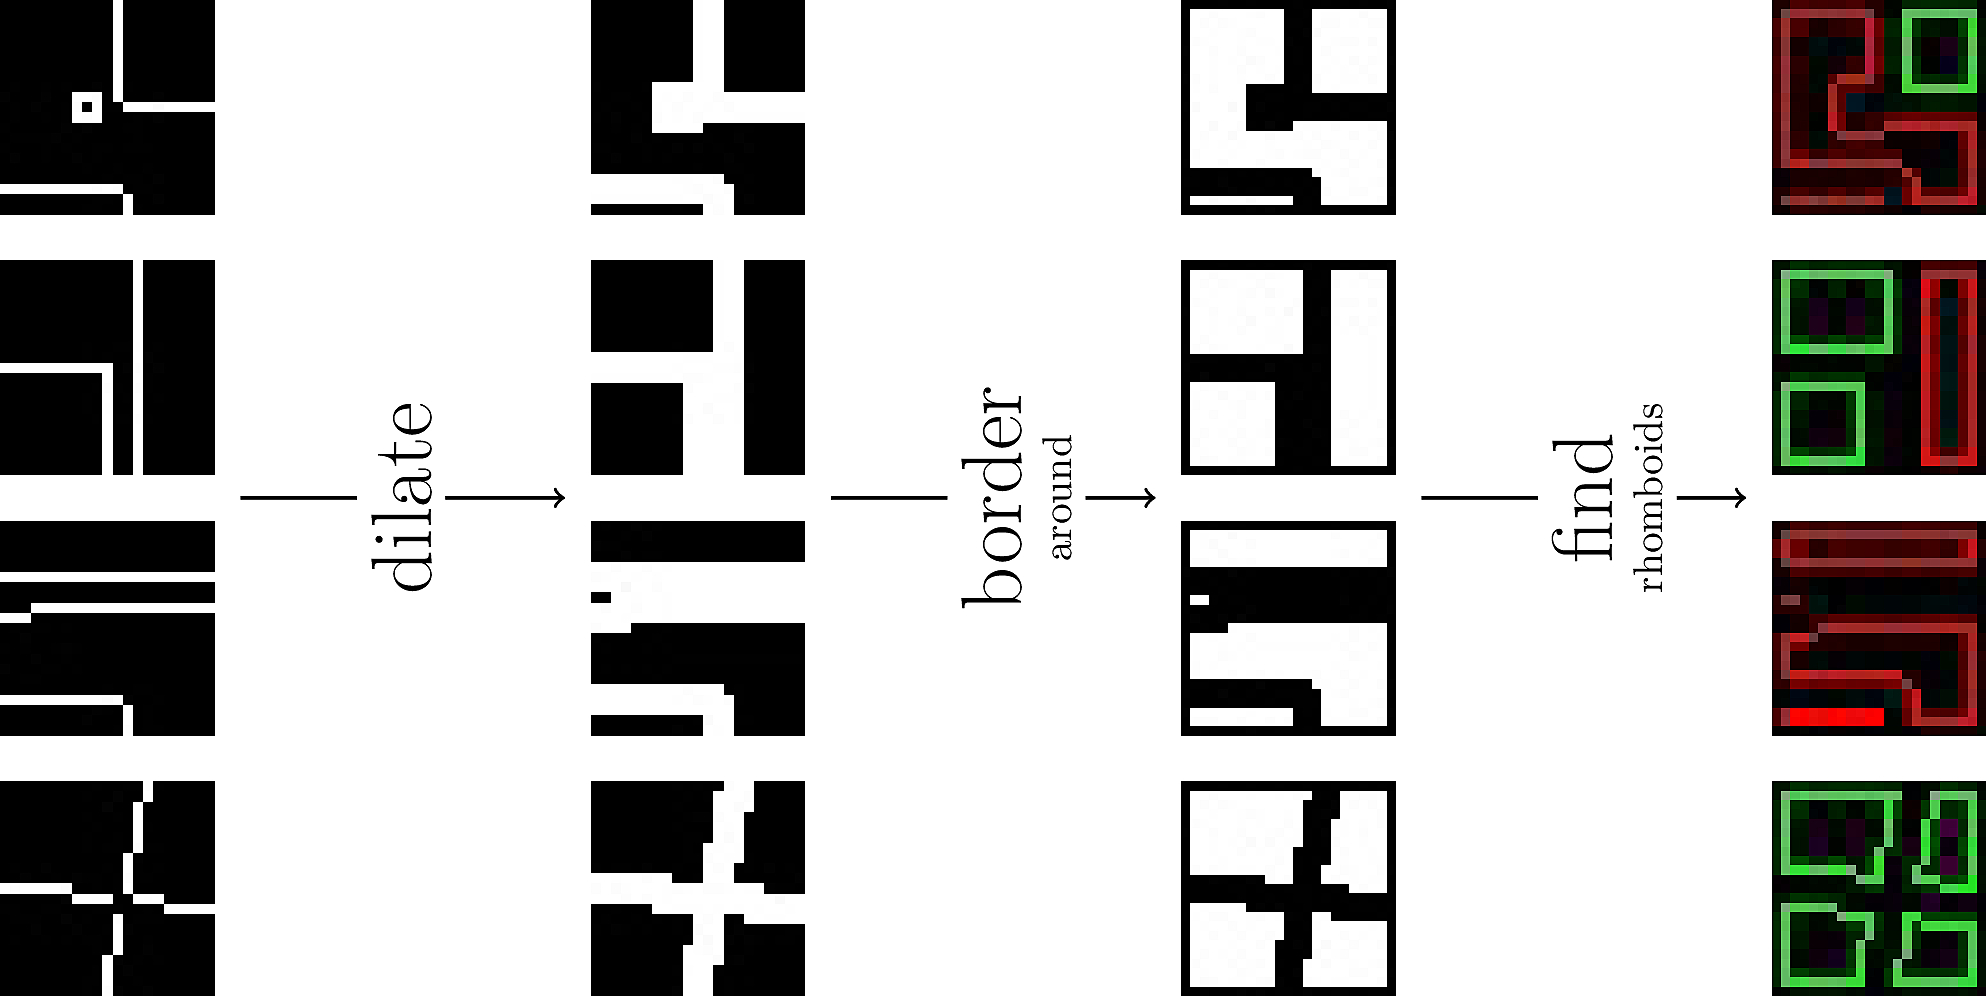
\includegraphics[width=\columnwidth]{figure7}
\caption{visualization how geometric PAMG classify vertice}
\end{figure}

After the checkered board is cut, all the lattice points can be divided into three categories: geometrically detected, neural detected, not detected.
Points not detected in the final phase are redone over the network. By repeating
this process on increasingly difficult chess-boards, the detector starts to
develop increasingly difficult combinations.

Theoretically, the PAMG could in this way learn any pattern.
You only need to create a ``geometrically'' perfect form of the pattern, then learn
from the simplest, most ideal to compiled unattainable examples (with which
human will not be able to handle).

\subsection{Reconstruct}

Our method use very primitive but effective technique to rebuild a grid.
We naively use the fact that the points that we manipulate belongs to a
regular grid. Thus, we present such a simplistic formula (density of the grid):

\[S = \dfrac{p^3}{x*\log_{10}{(x)}}\]

The value $p$ is number of points inside the frame, $x$ means surface area and $S$ means score. Larger score value is, than more regular grid you have found.
If you want to do it better you should get acquainted with
\cite{tian2011rectification}. However, when chess-board vertices detector returns
a lot of points, there is no need to do something with it.

\begin{figure}[H]
\centering
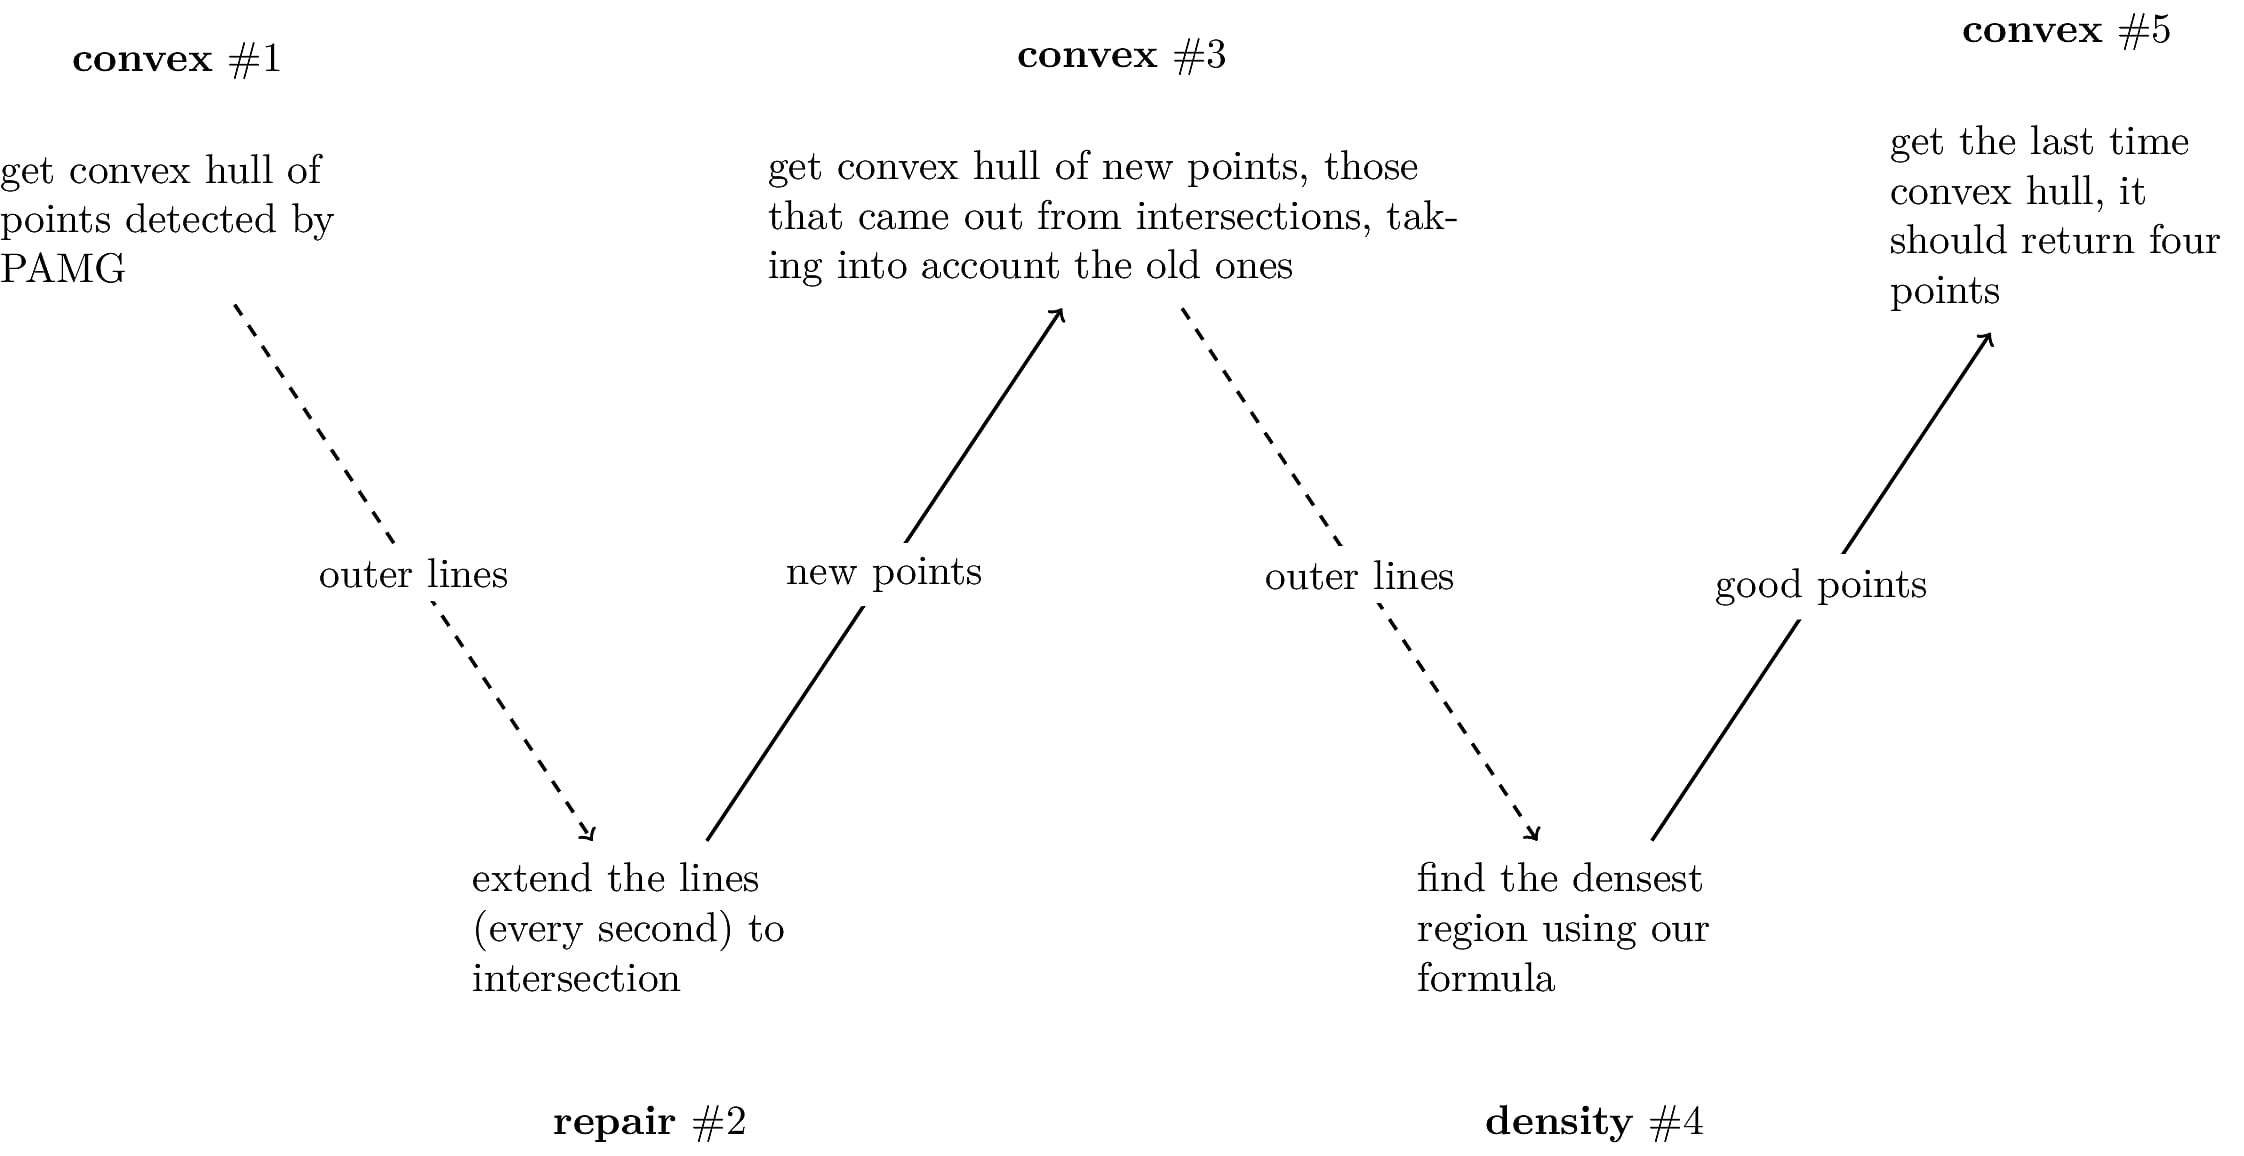
\includegraphics[width=\columnwidth]{figure8}
\caption{diagram showing primitive technique of grid reparation}
\end{figure}

\begin{figure}[H]
\centering
\subfigure[steps \#1-3]{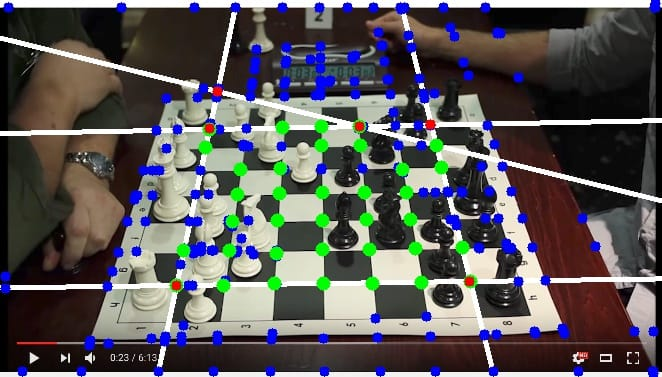
\includegraphics[width=0.48\columnwidth]{figure9a}}
\subfigure[steps \#3-5]{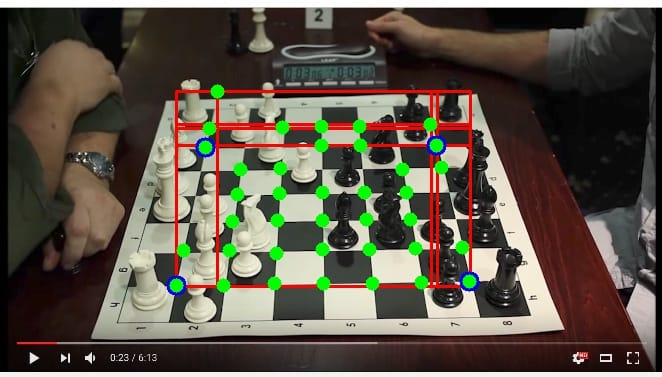
\includegraphics[width=0.48\columnwidth]{figure9b}}
\caption{visually presented algorithm's steps; red points are predicted}
\end{figure}

\subsection{Padcrop}

\begin{wrapfigure}{R}{0.25\textwidth}
\centering\vspace*{-0.6in}
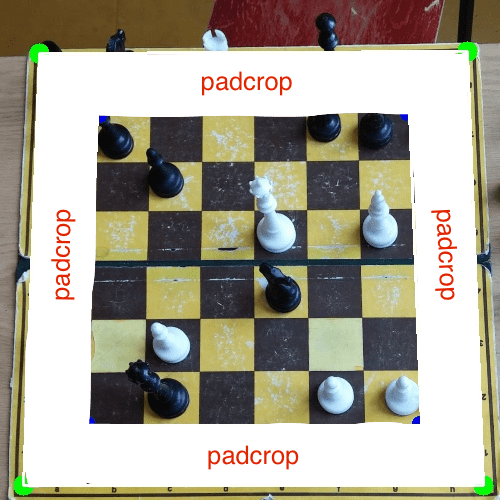
\includegraphics[width=\columnwidth]{figure10}
\caption{visually presented padcrop operation}
\end{wrapfigure}

Etymology of the word ``padcrop'' is simple; \textit{padcrop = padding + crop}. This operation is responsible for preparing the images for the next stage.
The difference is that the padding size is different at each stage. In our
implementation, at every stage padding was getting smaller (error value).

\[w/8/2 * (100 + \Delta) = 1000/8/2 * (100 + 0) = 62.5\]

The value $w$ is a width of
the image\footnote{that should be a square, thus height is the same} and $\Delta$
is the error, at the final step $\Delta$ should be 0.
Thus, it is easy to calculate the padcrop size for final stage (example above).

\section{Results}

\begin{figure}[H]
\centering
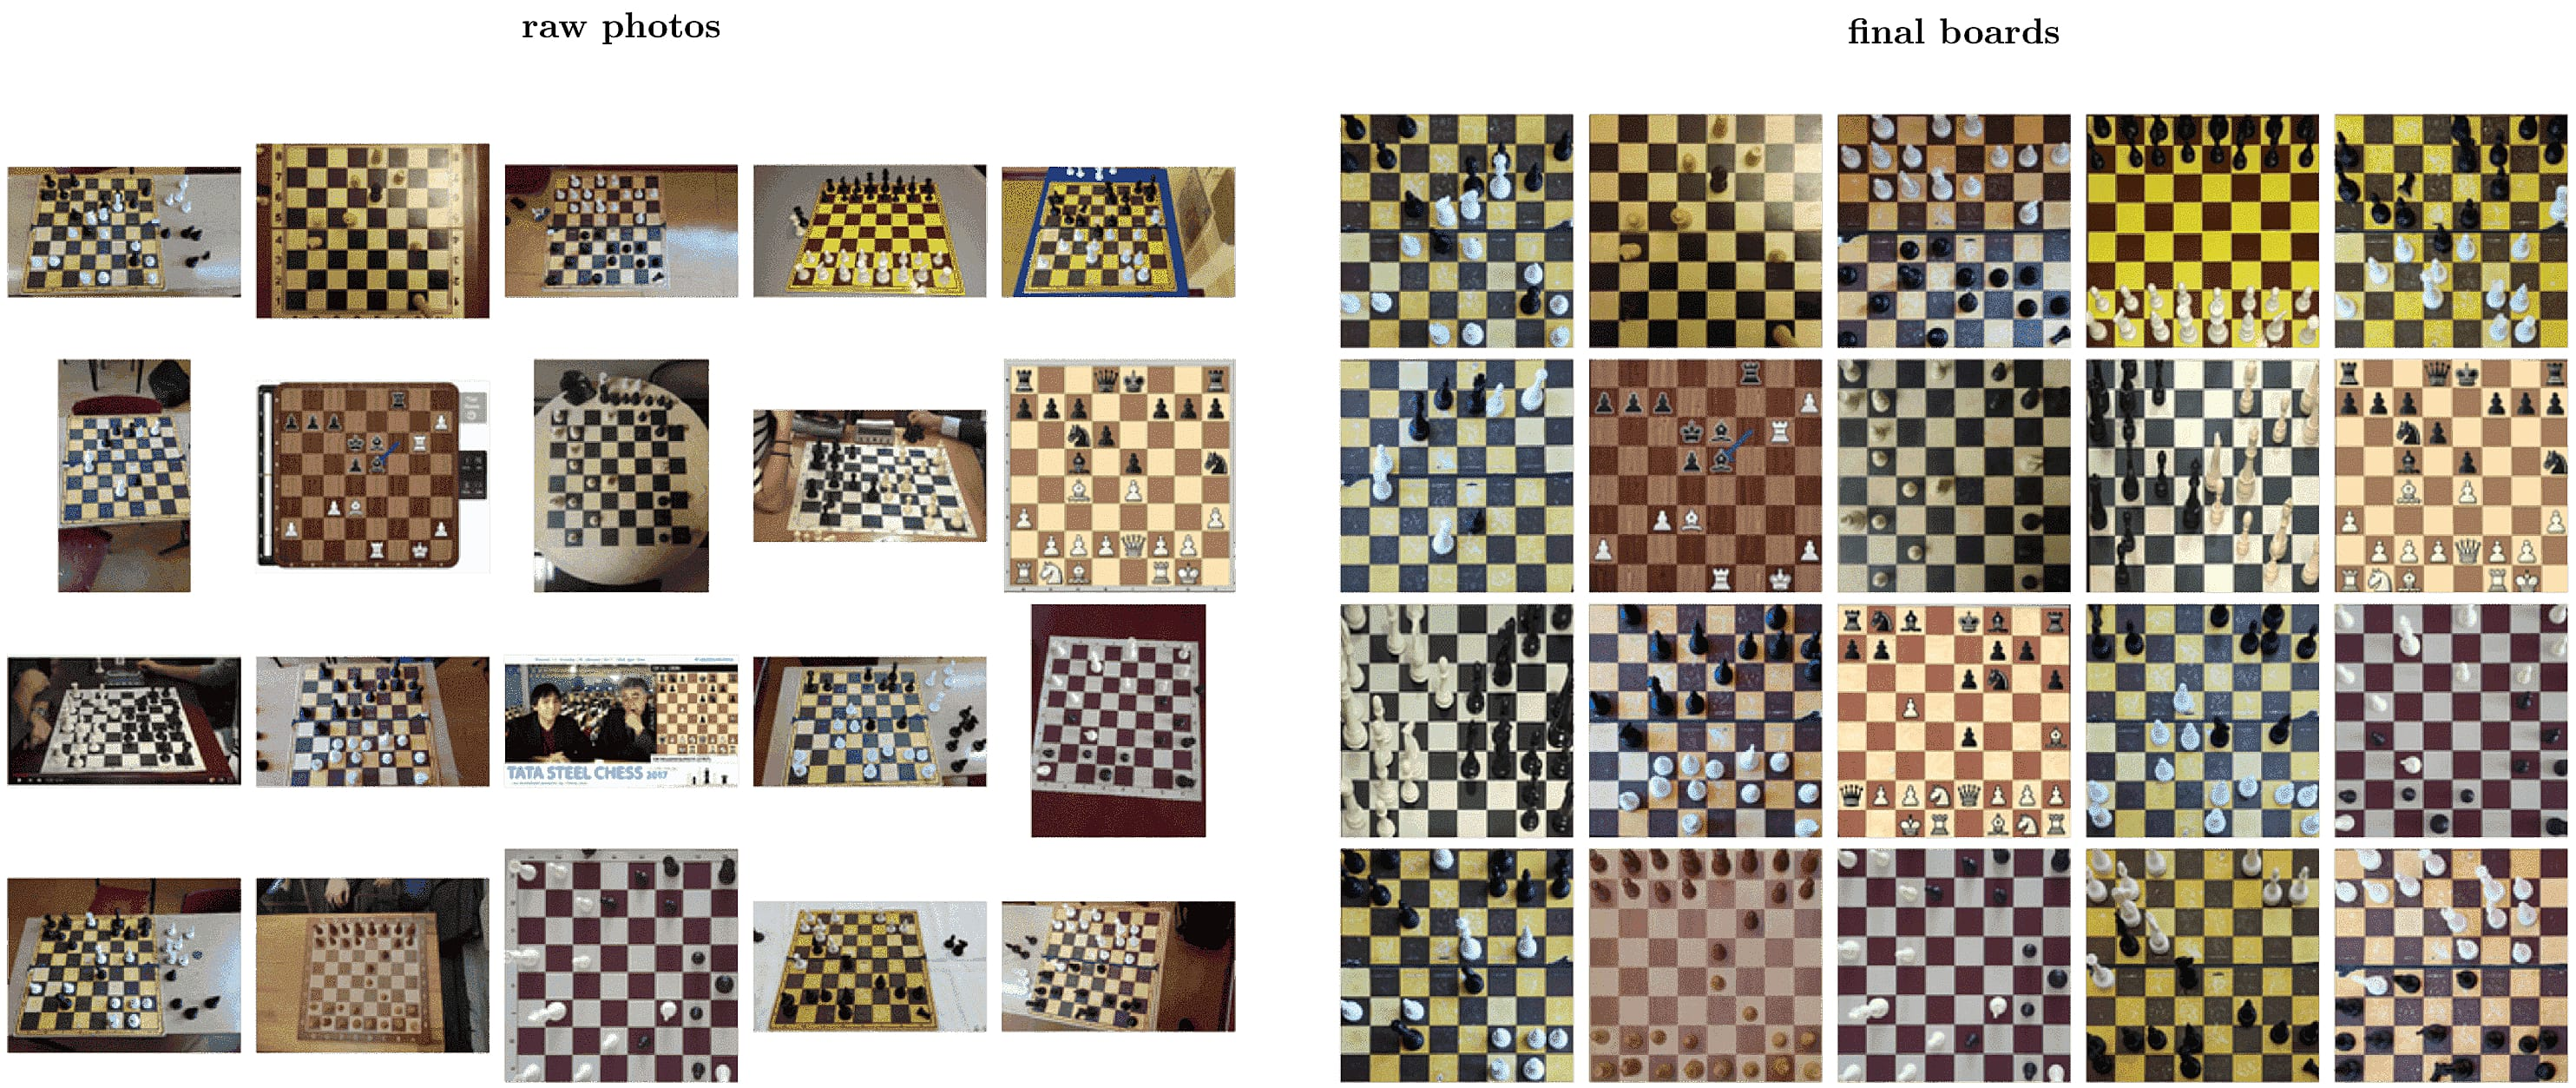
\includegraphics[width=\columnwidth]{figure11}
\caption{visually presented results, final boards ready for further analysis}
\end{figure}

In the picture above, we present the results visually.
The images were made using different devices, perspectives, chess-boards and positions.
The method is simple and does its job. Additionally, the method of subsequent matching avoids many mistakes at different
stages of program execution. In some difficult cases the second layer behave
badly. But in the final phase it usually returns to normal position. However, we suspect there must be a case that results would be totally wrong.
In the future, we plan to do more tests and possibly present even better techniques.

\begin{figure}[H]
\centering
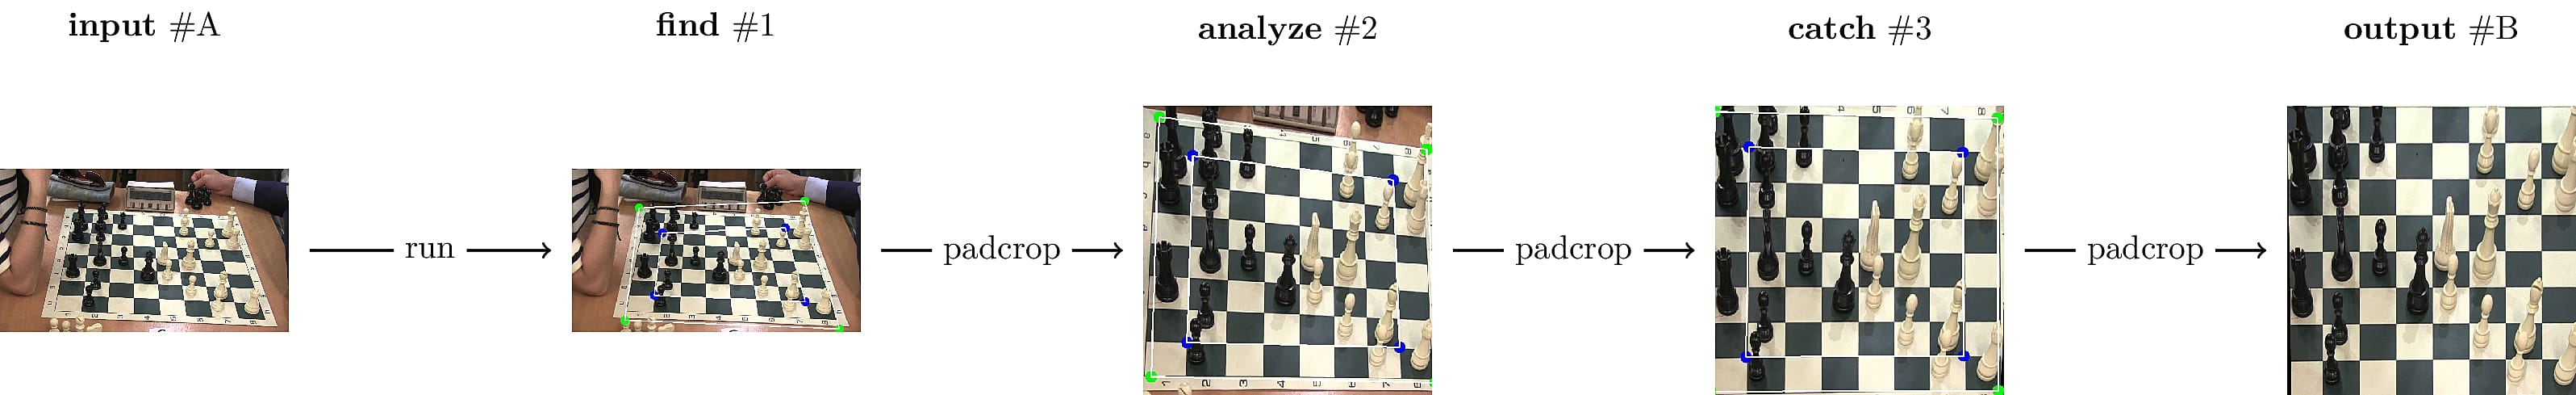
\includegraphics[width=\columnwidth]{figure12}
\caption{second layer looks terrible (cause King at \textit{b8}), however final product is okay}
\end{figure}

\section{Applications}

The PAMG and FAPL modules can be used independently, not only for cropping boards.
For example, we used the PAMG detector to find \textbf{ChArUco Corners}
\url{http://docs.opencv.org/3.1.0/df/d4a/tutorial_charuco_detection.html} with
better results than the default \textbf{Opencv} module.

\section{Conclusion}

Our method could help creating an automated system that
uses computer vision to provide insights into chess games played on physical boards.
We have used method described in \cite{dingchessvision} to digitize chess game.
In result, we have achieved better results than those obtained in
\cite{danner2015visual} (the method that was considered to be the most effective).

\begin{figure}[H]
\centering
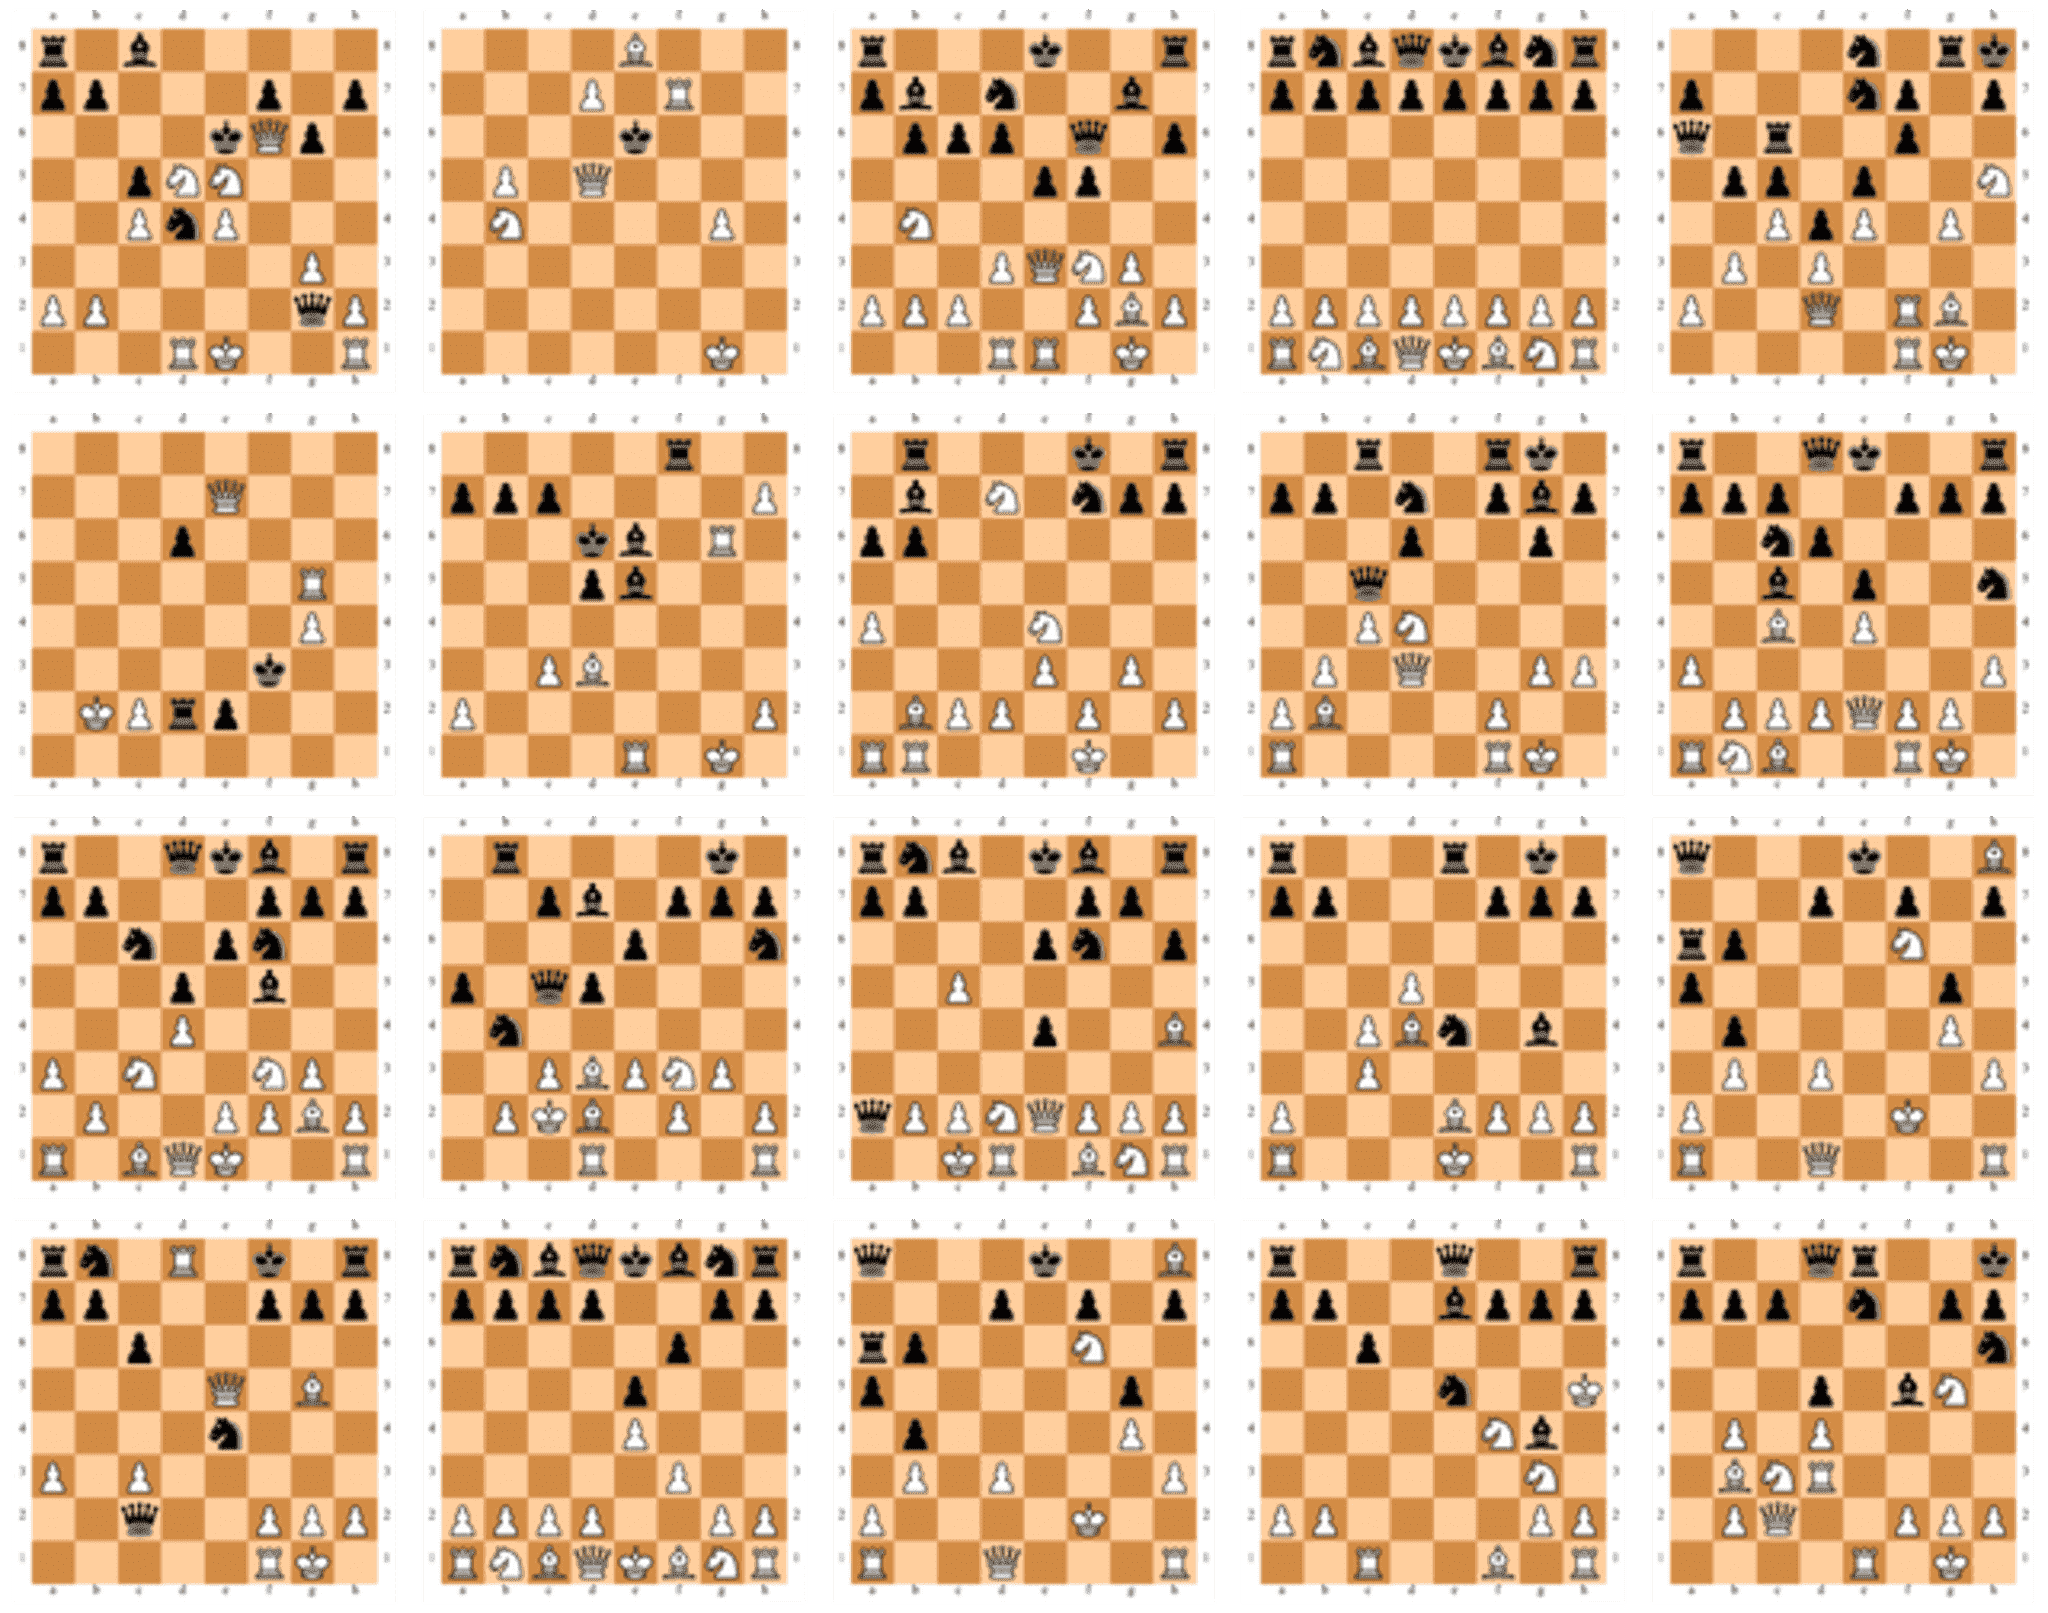
\includegraphics[width=0.6\columnwidth]{figure13}
\caption{FENs made using \cite{dingchessvision} method from cropped boards from
\textit{Figure 11}}
\end{figure}

\begin{figure}[H]
\centering
\subfigure[our crop + \cite{dingchessvision} chess-pieces]{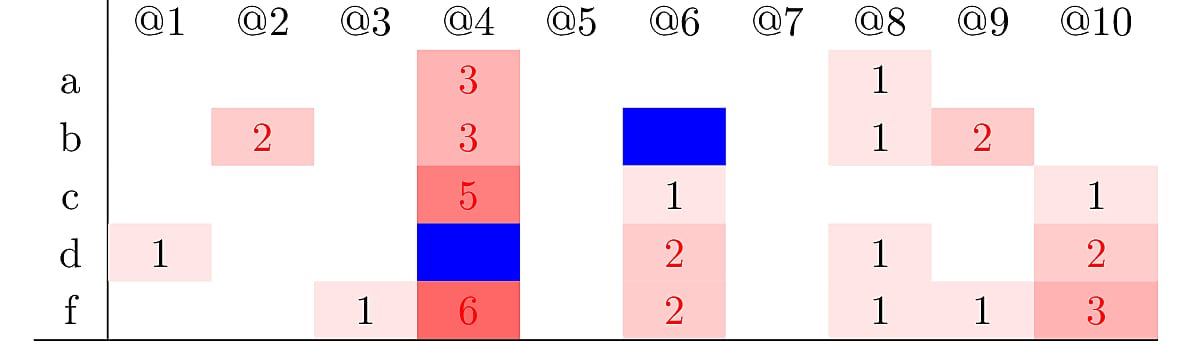
\includegraphics[width=0.48\columnwidth]{figure14a}}
\subfigure[\cite{danner2015visual} method]{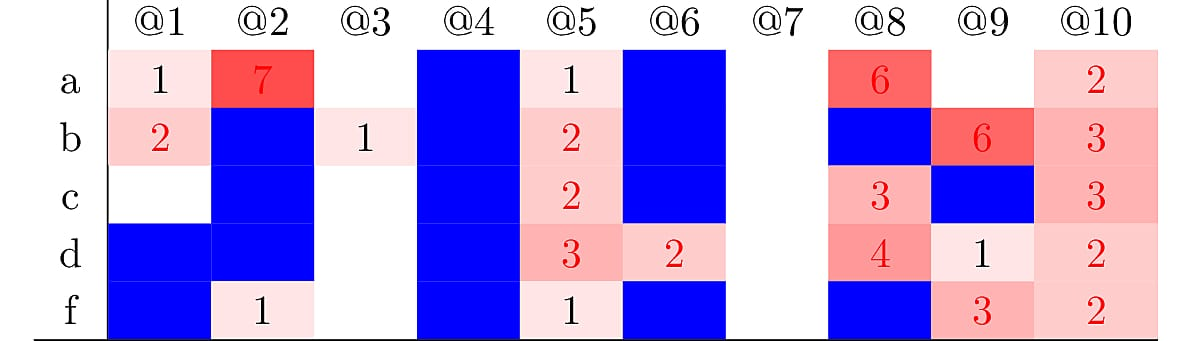
\includegraphics[width=0.48\columnwidth]{figure14b}}
\caption{we made \textit{@1-10} different chess positions and took \textit{a-f}
photos from different perspectives; numbers determine how many mistakes program
have made (wrong piece on the square); blue boxes means that not cropped properly;
our crop passed 96\% of test cases}
\end{figure}

%%%%%%%%%%%%%%%%%%%%%%%%%%%%%%%%%%%%%%%%%%%%%%%%%%%%%%%%%%%%%%%%%%%%%%%%%%%%%%%%%
%% BIBLIOGRAPHY
%%%%%%%%%%%%%%%%%%%%%%%%%%%%%%%%%%%%%%%%%%%%%%%%%%%%%%%%%%%%%%%%%%%%%%%%%%%%%%%%%

\printbibliography[title={References}]

%%%%%%%%%%%%%%%%%%%%%%%%%%%%%%%%%%%%%%%%%%%%%%%%%%%%%%%%%%%%%%%%%%%%%%%%%%%%%%%%%
%% APPENDIX
%%%%%%%%%%%%%%%%%%%%%%%%%%%%%%%%%%%%%%%%%%%%%%%%%%%%%%%%%%%%%%%%%%%%%%%%%%%%%%%%%

\clearpage\appendix

\section{Raw Process (Maurice Ashley)}

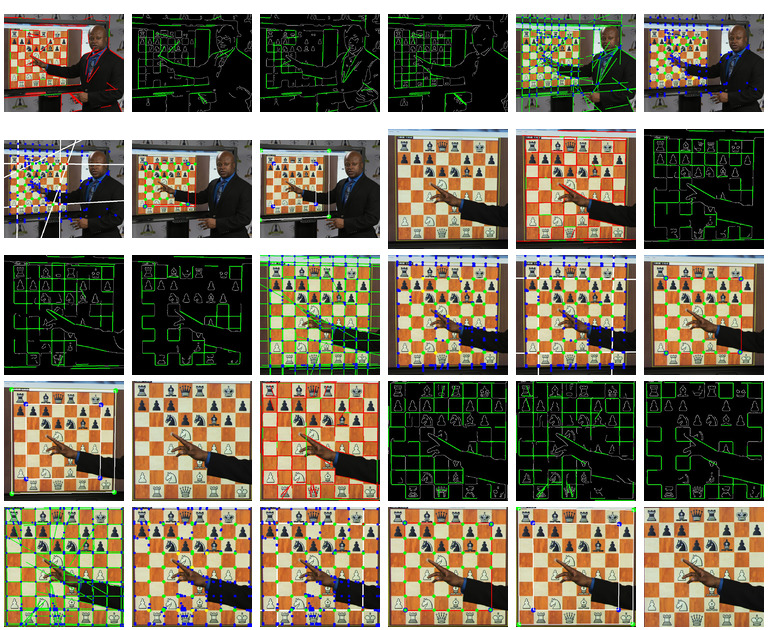
\includegraphics[width=\columnwidth]{appendixA}
\clearpage

\section{PAMG Neural Network}

\begin{lstlisting}
from tflearn.layers.core import input_data,dropout,fully_connected
from tflearn.layers.conv import conv_2d,max_pool_2d,highway_conv_2d
from tflearn.layers.normalization import local_response_normalization, \
                                         batch_normalization
from tflearn.layers.estimator import regression

def pamg_neural_network():
    """PAMG - experimental neural network for regular patterns/structures"""

    # input
    net = input_data(shape=[None, 21, 21, 1], name='input')

    # H(2)
    for i in range(2):
        for j in [3, 2, 1]:
            net = highway_conv_2d(net, 16, j, activation='elu')
        net = max_pool_2d(net, 2)
        net = batch_normalization(net)

    # 2D(32)
    net = conv_2d(net, 32, 3, activation='relu', regularizer="L2")
    net = max_pool_2d(net, 2)
    net = local_response_normalization(net)

    # 2D(64)
    net = conv_2d(net, 64, 3, activation='leaky_relu', regularizer="L2")
    net = max_pool_2d(net, 3)
    net = local_response_normalization(net)

    # 2D(128)
    net = conv_2d(net, 128, 3, activation='relu6', regularizer="L2")
    net = max_pool_2d(net, 4)
    net = local_response_normalization(net)

    # F(128)
    net = fully_connected(net, 128, activation='elu')
    net = dropout(net, 0.5)

    # F(256)
    net = fully_connected(net, 256, activation='tanh')
    net = dropout(net, 0.5)

    # output
    net = fully_connected(net, 2, activation='softmax')
    return regression(net, optimizer='adam', learning_rate=0.003,
                        loss='categorical_crossentropy', name='target')
\end{lstlisting}

%%                               END OF DOCUMENT                               %%
%%%%%%%%%%%%%%%%%%%%%%%%%%%%%%%%%%%%%%%%%%%%%%%%%%%%%%%%%%%%%%%%%%%%%%%%%%%%%%%%%
%%%%%%%%%%%%%%%%%%%%%%%%%%%%%%%%%%%%%%%%%%%%%%%%%%%%%%%%%%%%%%%%%%%%%%%%%%%%%%%%%

\end{document}
